\documentclass[12pt]{article}

\usepackage{scicite,times,graphicx,float,hyperref}
\usepackage[skip=0pt]{caption}

\topmargin -1.0cm
\oddsidemargin 0.0cm
\textwidth 16cm 
\textheight 23cm
\footskip 1.0cm

\newenvironment{sciabstract}{%
\begin{quote} \bf}
{\end{quote}}

\newcounter{lastnote}
\newenvironment{scilastnote}{%
  \setcounter{lastnote}{\value{enumiv}}%
  \addtocounter{lastnote}{+1}%
  \begin{list}%
  {\arabic{lastnote}.}
  {\setlength{\leftmargin}{.22in}}
  {\setlength{\labelsep}{.5em}}
}
{\end{list}}

\title{Lab Work 2} 

\author
{André Pedrosa [85098], Filipe Pires [85122], João Alegria [85048]\\
\\
Algorithmic Information Theory\\
\normalsize{Department of Electronics, Telecommunications and Informatics}\\
\normalsize{University of Aveiro}\\
} 

\date{\today{}}

%%%%%%%%%%%%%%%%% END OF PREAMBLE %%%%%%%%%%%%%%%%

\begin{document} 

\baselineskip18pt

\maketitle 

\section*{Introduction}

This report aims to describe the work developed for the second assignment
of the course of 'Algorithmic Information Theory', explaining all programs
developed by us, and presenting the results we considered most relevant 
regarding the quality of the solutions. 

The programs implemented in C++ have the purpose of analysing and encoding
audio files and ultimately being capable of, from a small audio sample, 
identifying the music that it most likely belongs to.

Along with the description of the solution, we also discuss the effects
of the variation of the programs' parameters and how accurate are the results.
All code developed is publicly accessible in our GitHub repository:
\url{https://github.com/joao-alegria/TAI} .
\newpage

\section*{1. Data Visualization}

In this chapter we present a description of the dataset used, the small script 
we developed to convert audio samples from stereo to mono and the histograms
we are capable of plotting by adapting one of the scripts given along with the
assignment's description \cite{trab1}.

\subsection*{1.1. Dataset}

We were given the access to a small dataset containing 7 audio samples from 
different musics. It was these samples we used to test all our code.
Each audio file is in \texttt{.wav} format and has two signal channels (stereo).
They vary between 13 and 29 seconds of audio and, when played, none seems to 
contain significant noise.

\subsection*{1.2. Mono Conversion}

One of the tasks proposed was to create a script that converts stereo audio 
files into mono.
This was fairly straightforward to do, as it only required for us to read the v
alues from all signal channels and calculate the average of each.
The script is executed in the format presented below, once built:

\begingroup
\addtolength\leftmargini{-0.4in}
\begin{quote}
\begin{verbatim}
$ ./wavquant inputFile outputFile [-q quantSize] [-r reductFactor]
\end{verbatim}
\end{quote}
\endgroup

This script, \texttt{wavquant.cpp}, is also used for other purposes, in which 
the \texttt{quantSize} and \texttt{reductFactor} parameters are useful.
For this reason, we made the parameters optional, so that a user can run 
\texttt{wavquant} to simply convert stereo files into mono, with a default 
number of bits used to encode each value of the sample of 16 and no frequency
reduction factor.
This script is mentioned further ahead in greater detail.

\subsection*{1.3. Histograms}

We were also given a script called \texttt{wavhist.cpp} that outputted to the 
terminal the histogram of an audio file.
We adapted this script so that it accepts audio files (either stereo or mono) 
and plots in a figure the histogram of one of the audio channels.
The script uses \texttt{gnuplot} \cite{gnuplot}, a portable command-line driven 
graphing utility, and has the following format:

\begingroup
\addtolength\leftmargini{-0.4in}
\begin{quote}
\begin{verbatim}
$ ./wavhist inputFile channel
\end{verbatim}
\end{quote}
\endgroup

Figures \ref{fig:histogram_stereo} and \ref{fig:histogram_mono} contain the 
histograms plotted from the same music in the original format (stereo) and after 
its conversion to mono. 
The x axis represents the frequency of the values and the yaxis the number of 
occurences in the music of each frequency.

\begin{figure}[H]
  \centering
  \begin{minipage}{.5\textwidth}
    \centering
    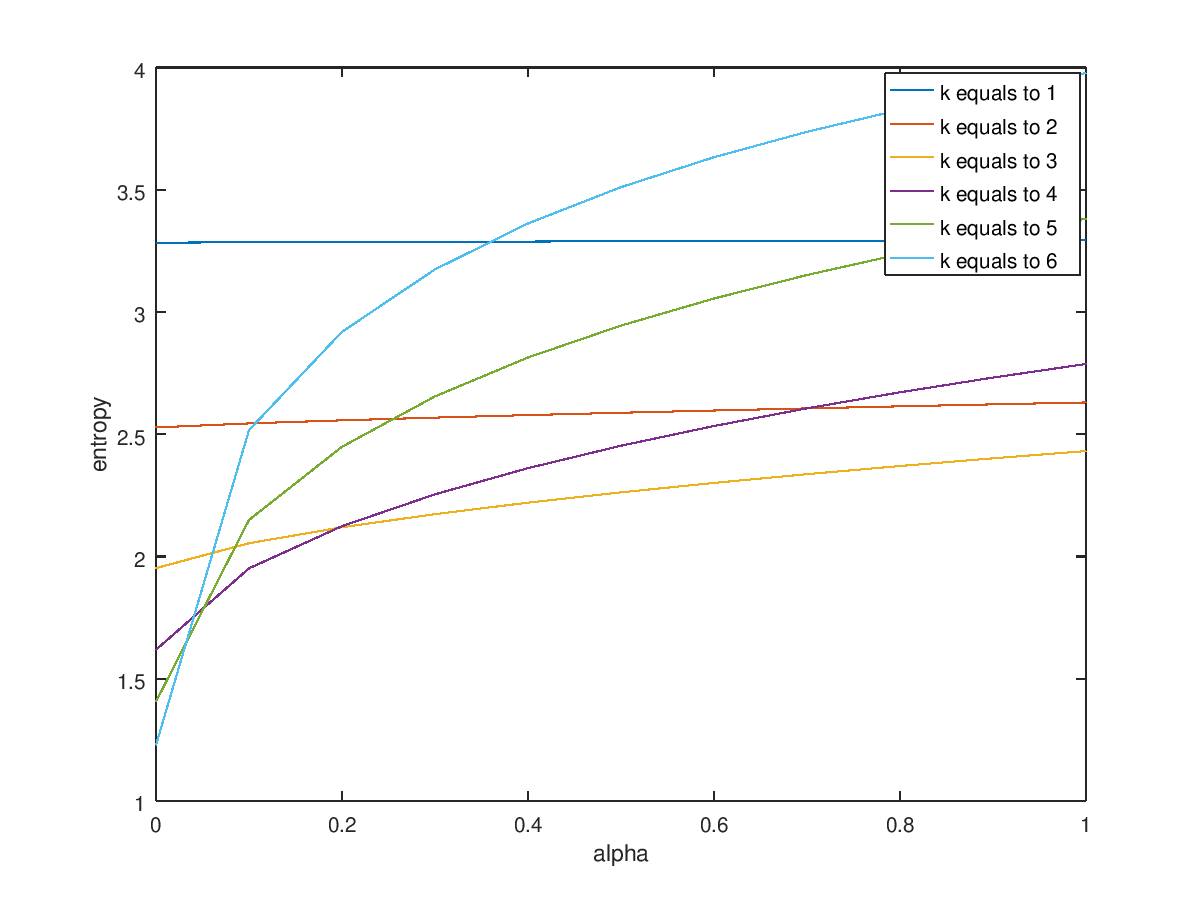
\includegraphics[width=\linewidth]{bible_en.png}
  \end{minipage}%
  \begin{minipage}{.5\textwidth}
    \centering
    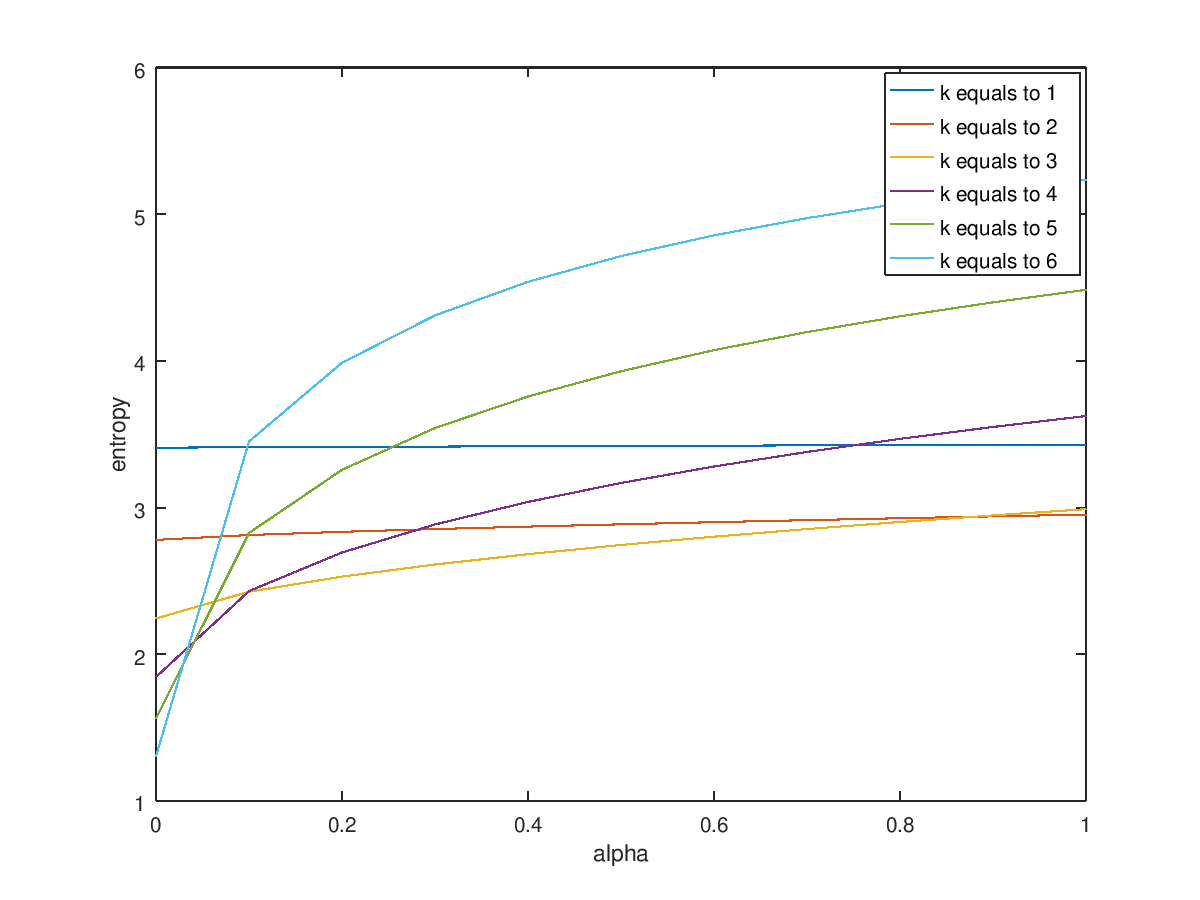
\includegraphics[width=\linewidth]{bible_pt.png}
  \end{minipage}
  \caption{Histogram of music\_name in the original format - channels 0 and 1.}
  \label{fig:histogram_stereo}
  
  \centering
  \begin{minipage}{.5\textwidth}
    \centering
    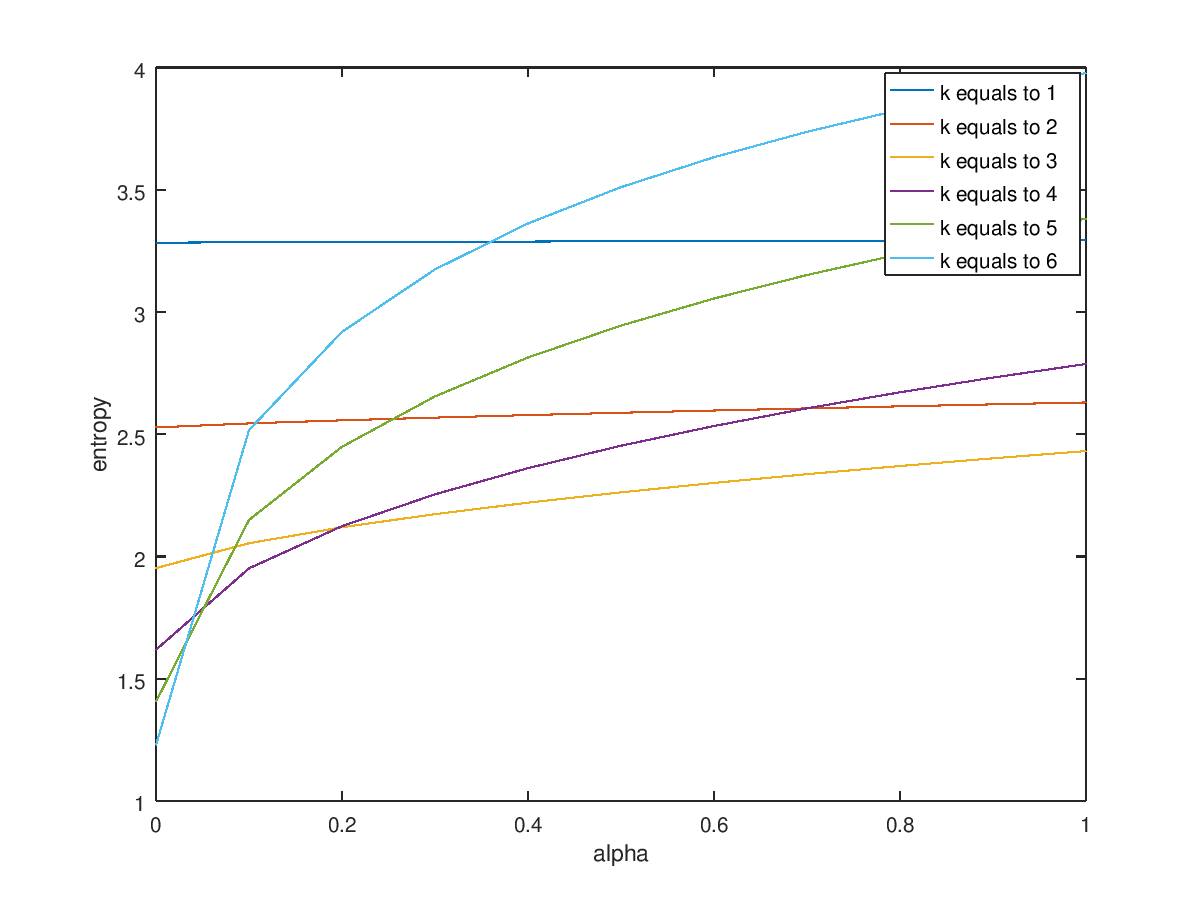
\includegraphics[width=\linewidth]{bible_en.png}
  \end{minipage}%
  \caption{{Histogram of music\_name after its conversion to mono (1 channel only).}}
  \label{fig:histogram_mono}
\end{figure}

............

Try to reduce the space between figure and caption

Mention something about why do the shapes are as they are and why is mono so different

............

The C++ scripts mentioned in this chapter all use \texttt{libsndfile}, a C 
library used for reading and writing files containing sampled sound \cite{libsndfile}.
This was proposed on the assignment and allowed us to read and manipulate the 
audio files for more complex tasks.

\newpage
\section*{2. Data Processing}

Once we were capable of visualizing the data, we proceeded to actually doing 
something useful with it.
In this chapter we explain the implementation of the program \texttt{wavquant.cpp},
responsible for reducing the number of bits used to represent each audio sample.
The implementation of the formulas presented on the assignment's description for
the signal-to-noise ratio and the energies of the signals and noises is described
as well, along with the computation of vector quantization codebooks of audio files.

\subsection*{2.1. Uniform Scalar Quantization}

The idea behind a uniform scalar quantization (USQ) is the reduction of bits 
used to represent a signal.
Its usage has an instrinsic tradeoff between signal quality and memory space
required to store the information.
We do not get into much detail regarding the mathematics behind this process, 
but we make available a figure taken from a presentation from the Stanford 
University \cite{stanford} that helps visualizing the outcome of applying the 
USQ to a signal.
Figure \ref{fig:quantization} contains a signal presented in blue and the outcome
of the signal after it is quantized is presented in red. 
The figure also contains the quantization error variation on
the second plot.

\begin{figure}[H]
  \centering
  \begin{minipage}{\textwidth}
    \centering
    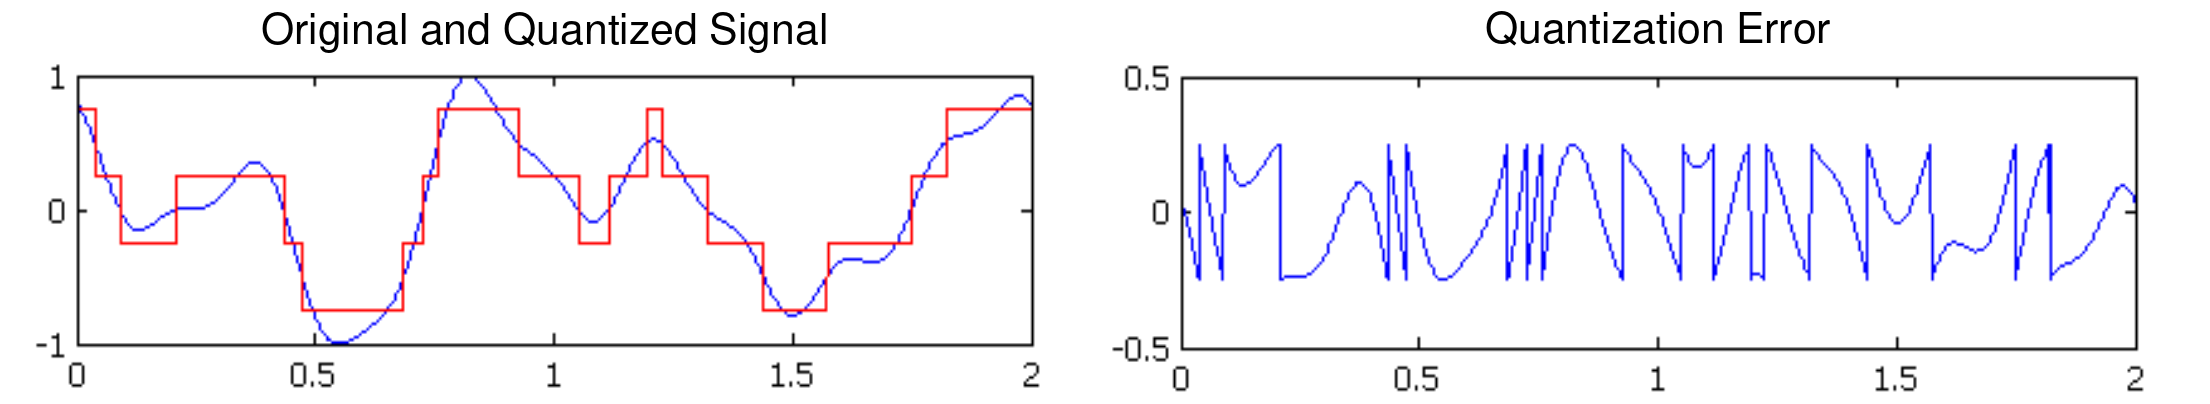
\includegraphics[width=\linewidth]{stanford_quantization_wide.png}
  \end{minipage}%
  \caption{Example of a quantized waveform.}
  \label{fig:quantization}
\end{figure}

It is the \texttt{wavquant.cpp} that is responsible for this process.
As we have seen in Section 1.2, the script accepts two optional parameters:
\texttt{quantSize} defines the number of bits to be used to represent the audio 
sample given as input (ideally, this value should be less than of the original 
sample); \texttt{reductFactor} defines the number of times the user would like 
to reduce the total number of values of the sample.
This reduction factor works by calculating the average between \texttt{n} values, 
where \texttt{n = reductFactor}, and doing this for all values from the sample.
The result is a sample with \texttt{n} times less values.

\subsection*{2.2. Error Calculation}

...

\subsection*{2.3. Vector Quantization Codebook}

...

\subsection*{2.4. Codebook Parallel Processing}

...

\newpage
\section*{3. Automatic Music Identification}

The program \texttt{wavfind.cpp} is the application of the previous scripts on a 
program with a specific purpose.
WAVFind is ment to interpret an audio sample and attempt to identify which music 
from a database it belongs to.
In this chapter we discuss our solution, the consequences fo varying the 
parameters passed to it and the quality of the results.

\subsection*{3.1. Most Probable Music}

...

\subsection*{3.2. Parameters Variation}

...

\subsection*{3.3. Results Discussion}

...

\newpage
\section*{Conclusions}

After completing the assignment, we drew a few conclusions regarding our 
solutions and the applicability of algorithms such as the K-Means to solving
problems such as music identification.

First of all, ...

Regarding our satisfaction with the delivered code,...

Finally, in terms of code organization and readability, we made sure our 
repository was as well structured as possible and our code properly commented
and documented.
The base folder contains a {\it README\/} file for basic instructions and a 
{\it Makefile\/} to make the compilation process easier.
All code is in the {\it src\/} folder and its documentation is accessible, 
with the help of the {\it Makefile\/} and the command "make docs", through
the automatically generated {\it index.html\/} file in the {\it docs\/} 
directory.

\begin{thebibliography}{9}
  \bibliographystyle{Science}

  \bibitem{trab1}
    Armando J. Pinho,
    \textit{AIT: Lab Work no.2},
    University of Aveiro,
    2019/20.
  
  \bibitem{gnuplot}
    H.B. Broeker, G. Clark, L. Hecking and E. Merritt,
    \textit{Gnuplot: graphing utility},
    \url{http://www.gnuplot.info/} ,
    May 2019,
    [accessed in: November 2019].

  \bibitem{libsndfile}
    Free Software Foundation,
    \textit{GLibsndfile API},
    \url{http://www.mega-nerd.com/libsndfile/api.html} ,
    April 2013,
    [accessed in: November 2019].

  \bibitem{stanford}
    Bernd Girod,
    \textit{Image and Video Compression: Quantization},
    \url{https://web.stanford.edu/class/ee398a/handouts/lectures/05-Quantization.pdf} ,
    [accessed in: November 2019].

    

\end{thebibliography}

\clearpage

\end{document}




















